\documentclass{article}
\usepackage[utf8]{inputenc}
\usepackage{xcolor}
\usepackage{multicol}
\usepackage[notes=true,draft]{dtrt}
\usepackage[margin=1in]{geometry}
\usepackage{tikz}
\usetikzlibrary{graphs,graphs.standard,shapes.geometric, arrows}
\usepackage{caption}
\usepackage{subcaption}
\usepackage{fontawesome}
\usepackage[operators]{cryptocode}
\usepackage{amsmath}
\usepackage{amssymb}
\usepackage{fancyvrb}


\title{Comm}
\author{Technical Whitepaper}
\date{}

% -------------------------------

\newcommand{\sk}{{\sf sk}}
\newcommand{\pk}{{\sf pk}}
\newcommand{\pw}{{\sf password}}
\newcommand{\signauth}{{\sf sign}_{\sf auth}}
\newcommand{\signbackup}{{\sf sign}_{\sf backup}}
\newcommand{\msgauth}{{\sf msg}_{\sf auth}}
\newcommand{\msgbackup}{{\sf msg}_{\sf backup}}

\newcommand{\id}{{\sf ID}}
\newcommand{\salt}{{\sf salt}}
\newcommand{\bk}{{\sf BackupKey}}
\newcommand{\bkdata}{{\sf BackupDataKey}}
\newcommand{\bid}{\sf BackupID}
\newcommand{\hmac}{\sf HMAC}
\newcommand{\hkdf}{\sf HKDF}
\newcommand{\keygen}{\sf Keygen}
\newcommand{\sign}{\sf Sign}
\newcommand{\signcomm}{\sf SignAndStampComm}
\newcommand{\verify}{\sf Verify}
\newcommand{\verifycomm}{\sf VerifyComm}
\newcommand{\sha}{\sf SHA256}
\newcommand{\bcrypt}{\sf bcrypt}
\newcommand{\aesenc}{\sf AEAD.Enc}
\newcommand{\aesdec}{\sf AEAD.Dec}
\newcommand{\ct}{\sf ct}
\definecolor{blue}{rgb}{0.25,0.25,1}
\definecolor{red}{rgb}{1,0.25,0.25}

\newcommand{\commsk}{{\sf CommSK}}
\newcommand{\commpk}{{\sf CommPK}}

\newcommand{\isk}{{\sf IdSecKey}}
\newcommand{\ipk}{{\sf IdPubKey}}
\newcommand{\csk}{{\sf PreSecKey}}
\newcommand{\cpk}{{\sf PrePubKey}}
\newcommand{\otsk}{{\sf OneTSecKey}}
\newcommand{\otpk}{{\sf OneTPubKey}}
\newcommand{\dl}{{\sf DeviceList}}
\newcommand{\isequal}{\stackrel{?}{=}}
\newcommand{\isin}{\stackrel{?}{\in}}

\newcommand{\wpk}{{\sf WalletPubKey}}

\newcommand{\userdata}{{\sf UserData}}
\newcommand{\userkeys}{{\sf UserKeys}}

\newcommand{\pdevice}{{\bf \color{red} Primary Device~}}
\newcommand{\udevice}{{\bf \color{magenta} User Device~}}
\newcommand{\comm}{{\bf \color{blue} Comm~}}
\newcommand{\afterauth}{{\bf \color{teal} After user authentication~}}

\newcommand{\aktodo}[1]{\dtcolornote[Anunay]{blue}{#1}}
\newcommand{\attodo}[1]{\dtcolornote[Ashoat]{red}{#1}}

% -------------------------------

\begin{document}

\maketitle

\noindent We describe the security architecture of the Comm platform and its component services. In the following sections, we limit the discussion of system design choices to only those with security or privacy implications.

\section*{Primitives}
\begin{itemize}
    \item $\sha$ is the Secure Hash Algorithm with 256 bit digests.
    \item $\hmac$ is a hash-based message authentication code initialized with $\sha$.
    \item TLS is the Transport Layer Security standard.
    \item OPAQUE is a password-authenticated key exchange (PAKE) protocol~\cite{opaque2018}.
    \item $\keygen$, $\sign(\sk, m)$, $\verify(\pk, m, \sigma)$ represent a secure digital signature algorithm (e.g., EdDSA, ECDSA). $\keygen$ returns a (private key, public key) pair and $\verify(\pk, m, \sigma) = \top$ if and only if  $\sigma = \sign(\sk, m)$ is a valid signature on message $\textsf{m}$.
    \item $\aesenc$, $\aesdec$ represent encryption and decryption functions respectively of an authenticated encryption scheme (e.g., AES-GCM).
    \item X3DH refers to the Extended Triple Diffie-Hellman key agreement protocol~\cite{x3dh}.
    \item $\signcomm(m)$ is a signing function used by Comm to sign message $m$ and the (then) current timestamp. For simplicity, we omit a full description of the signing process.
    \item SIWE refers to the Sign In with Ethereum standard described in Ethereum Improvement Proposal (EIP) 4361~\cite{siwe}.
\end{itemize}

\section*{Definitions}
\aktodo{Add context; Move to relevant sections}
\begin{itemize}
    \item $\commpk$ is a long-term public key used to verify Comm signatures. If $\sigma = \signcomm(m)$ is a valid signature on message $m$, $\verify(\commpk, m, \sigma) = \top$.
    \item Long-term identity key pair $(\isk, \ipk)$ is unique to each device. The identity key pair of the primary device does not change.
    \item Signed prekey pair $(\csk, \cpk)$ is unique to each device, rotated every month.
    \item A set of one-time prekey pairs $(\otsk_0, \otpk_0), \dots, (\otsk_9, \otpk_9)$, whose public keys are stored on Comm servers and replenished by user devices when required~\cite{signalprotocol}.
    \item $\wpk$ is the public key of the digital wallet used by a given user (Section \ref{sec:authenticationcomm}).
\end{itemize}

% \subsection*{Backup \& Restore}

\begin{itemize}
\item $\bk$ and $\bkdata$ are symmetric encryption keys used to encrypt $\userkeys$ and $\userdata$ respectively (Section~\ref{sec:backup}).

\item \userkeys~consists of identity key pairs of all devices associated with a given user, identity public keys used by all devices associated with all users that a given user has initiated a session with, and $\bkdata$.

\item \userdata~includes user-generated data including messages and media.

\end{itemize}

% \subsection*{Usability}
\begin{itemize}
\item \dl~is a list of pairs of identity public keys of all devices associated with a given user (Section~\ref{proto:dlupdate}). Each device has two long-term identity key pairs used to protect messages and notifications respectively.
\end{itemize}

\section{Core Concepts}
\label{sec:core_concepts}

\textbf{Primary Device.} Every user on Comm has a primary device. This can either be a cell phone or a keyserver.\\

\noindent \textbf{Keyserver.} A keyserver is a primary device that can also host communities. Keyservers are necessary to host communities because they can handle background processing and respond to queries on-demand. As keyservers are self-hosted, Comm is not able to control who has access to the data on a keyserver. Multiple users can share the same keyserver.\\

\noindent \textbf{Communities.} Communities in Comm are like servers in Discord. Each community is hosted on a specific user's keyserver. Users in Comm can be a member of any number of communities. Users in Comm can be a member of any number of communities.\\

\noindent \textbf{Chats.} There are two distinct kinds of chats in Comm.
\begin{itemize}
    \item \textbf{DMs.} DMs are similar to chats in iMessage, WhatsApp, or Signal. When you send a message to a local thread, your primary device encrypts that message separately for each recipient, and then sends it directly to each recipient.
    \item \textbf{Communities and channels.} Chats inside a community are called channels, and they are similar to channels in Slack or Discord. When you send a message to a channel, your primary device encrypts that message for the community host's keyserver, and the community host's keyserver handles sending it to participants. Because they are hosted on a keyserver, channels support more features than DMs.
\end{itemize}

\noindent \textbf{Threads.} Threads in Comm are like threads in Slack or Discord. They are created in response to a message in a parent thread. They can exist in both DMs and channels.


\section{Threat Model}
\label{sec:threatmodel}

We begin by defining types of user devices and chats supported by Comm.

\paragraph{Chats.} Comm supports two kinds of chats: direct chats and communities. Communities offer messaging channels (similar to Slack and Discord); direct chats do not. Both kinds of chats support Slack-like threading.

% Ashoat notes: check out https://www.notion.so/commapp/How-Comm-works-d6217941db7c4237b9d08b427aef3234

\begin{itemize}
    \item Direct chats are encrypted using a double ratchet~\cite{drsecurity}. No single device is considered the host of a direct chat, and instead each user device participates on the same level. See Section \ref{sec:usability} for details.
    \item Community data are encrypted in transit between the community's hosting keyserver and all user clients using keys derived from X3DH agreements. This not only ensures integrity and confidentiality but also allows streamlined authentication (see Section~\ref{sec:authenticationkeyserver}). Communities are hosted on a keyserver (see below), and rely on that keyserver's query response and background processing capabilities to provide richer functionality than is possible with direct chats. For example, communities support shared applications (e.g., calendars) and consist of discrete messaging channels.
\end{itemize}

\paragraph{Group Direct Chats.} In case of a direct chat involving more than two users, a double ratchet is constructed for every pair of devices used by each participant (Figure~\ref{fig:directchats}).

\begin{figure}[htb!]
    \centering
     \begin{subfigure}[b]{0.49\textwidth}
         \centering
         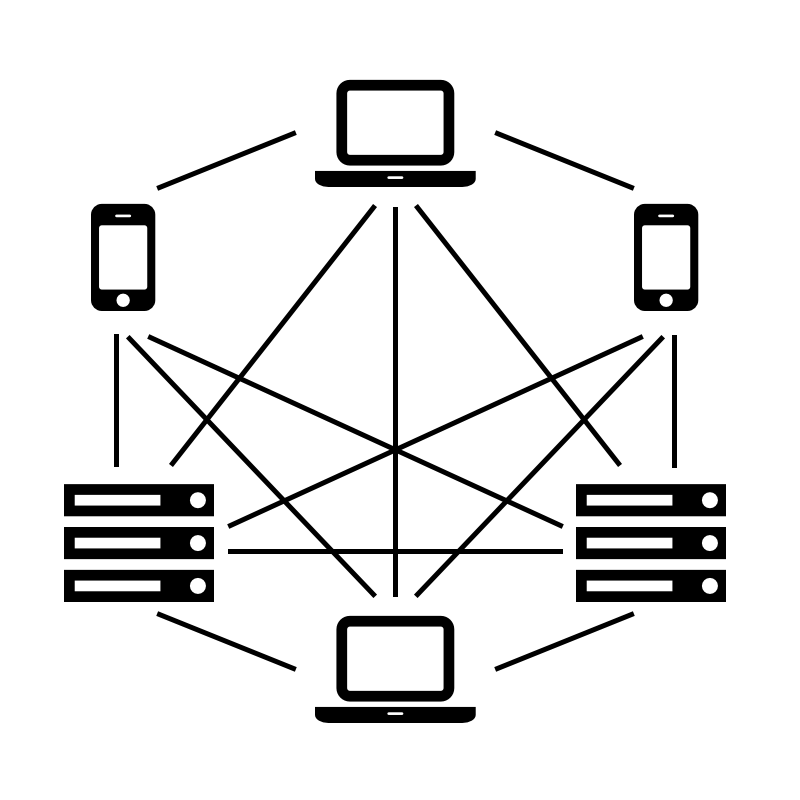
\includegraphics[width=\textwidth]{img/1a.png}
         \caption{Network communication pattern in a direct chat with six user devices.}
         \label{fig:directchats}
     \end{subfigure}
     \hfill
     \begin{subfigure}[b]{0.49\textwidth}
         \centering
         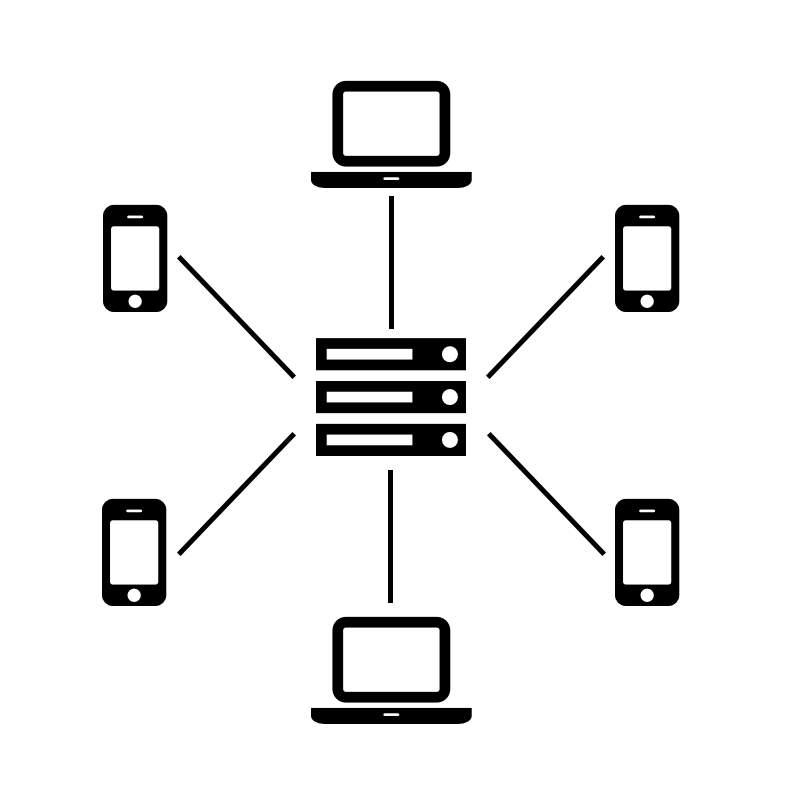
\includegraphics[width=\textwidth]{img/1b.png}
         \caption{Network communication pattern in a community with six user devices.}
         \label{fig:communities}
     \end{subfigure}
\end{figure}

\paragraph{User Devices.} The Comm system consists of two kinds of user devices: keyservers and clients.

\paragraph{Keyservers.} A keyserver is a user device that can respond to queries on-demand and execute background processing jobs. A user's keyserver functions as the backend for their applications. Comm does not host user keyservers, but supports various different models for deploying them (e.g., self-hosting, cloud hosting). A user can have up to one keyserver. Communities are always hosted on a keyserver but Comm also supports users running keyservers without any communities on them. A personal keyserver can benefit a user by syncing with all of the user's communities' keyservers in the background. However, not all Comm users need to host a keyserver.

For example, if a user is a member of 10 distinct communities, they need to connect to 10 keyservers when they open the Comm client on their mobile device. If they run their own keyserver, they can connect to just that one, since their keyserver can sync with the other keyservers in the background.

\paragraph{Clients.} Examples of clients include iOS, Android, and web clients. Unlike keyservers, clients are limited in their capacity for background processing, and cannot reliably respond to queries from other devices.

\paragraph{Primary Device.} The initial device used by a user to register for Comm is termed their primary device. The identity key pair of the primary device never changes and is restored from backup. The user can register new additional devices using the primary device. The primary device can only be switched under special circumstances (see Section~\ref{sec:usability}).


\subsection{Security}

\paragraph{Internal Threats.} An adversary that corrupts a Comm employee with access to PAKE data stored on Comm servers could change the value associated with a particular user. While this does not leak the user's password or password-equivalent data, it may allow the adversary to impersonate the user. Such attacks can be mitigated by using wallet-based authentication (see Section \ref{sec:authenticationcomm}).

\paragraph{Backups.} User backups cannot be decrypted without access to the user's password or wallet secret key (see Section \ref{sec:backup}).

\section{Authentication}

User devices authenticate either to Comm servers or to keyservers hosting communities. We describe these authentication mechanisms separately. Both authentication protocols ensure forward secrecy and cryptographic deniability. In either case, the corresponding parties compute a shared ephemeral secret that is used to derive an encryption key for the subsequent session.

\paragraph{Social Proof of Identity.} If a user device authenticates to Comm servers using a digital asset wallet (e.g., SIWE~\cite{siwe}), a social proof of identity is generated, which allows the user to tie their wallet to Comm identity keys and prove their (wallet) identity to other Comm users.

\subsection{Authenticating to community keyservers}
\label{sec:authenticationkeyserver}

\aktodo{Change to peers, mention differences between keyservers and devices. Mention peers verify social proof of identity}

% Ashoat notes: we should probably mention social proof here

Community keyservers and client user devices authenticate each other using the Extended Triple Diffie-Hellman (X3DH) key agreement protocol. They generate a shared secret, which is used as the key to a key derivation function (KDF) with constant input. Both parties use output of the KDF as a symmetric key for encrypting the session after X3DH concludes.

Comm does not use mutual TLS (mTLS) for client-keyserver communication in order to avoid implementation complexity. Certificates are also not useful in this setting as immediate revocation is required. Recent OpenSSL vulnerabilities in mTLS highlight the dangers of expanding the attack surface. As X3DH is also used to initiate double ratchets for direct chats, this decision enforces uniformity of inter-device communication. 

\subsection{Authenticating to Comm}
\label{sec:authenticationcomm}

Comm servers allow user devices to authenticate in two ways. All communication is secured via TLS.

\begin{itemize}
    \item User knows a $\pw$
    \item User provides a digital signature $\signauth$ constructed by a digital asset wallet (e.g., SIWE~\cite{siwe})
\end{itemize}

\paragraph{Password-based.} Comm uses password authenticated key-exchange (PAKE) to authenticate users. Specifically, Comm servers engage user clients in the OPAQUE protocol~\cite{opaque2018}. Comm does not store password-equivalent data. Even if stored authentication data are compromised, any adversary with access to them will still need to mount an expensive brute-force search in order to impersonate a user. Using OPAQUE, users authenticate themselves without ever sending password-equivalent data.

\paragraph{Signature-based.} If a user uses a digital asset wallet, the wallet's signing functionality can be used to generate a valid signature on a specific message. The Comm mobile apps (iOS and Android) construct the message $\msgauth$---using a nonce provided by the Comm server---and forward the user to the wallet app to procure a signature $\signauth$ on it. Figure \ref{fig:authmessage} describes an example message $\msgauth$. Comm servers store users' wallet public key, authentication message $\msgauth$, and the associated signature $\signauth$. Replay attacks against Comm servers are repelled by nonce verification.

\begin{figure}[htb!]
    \centering
        \begin{Verbatim}[frame=single]
                comm.app wants you to sign in with your Ethereum account:
                
                0xC02aaA39b223FE8D0A0e5C4F27eAD9083C756Cc2

                
                Device IdPubKey: 0x4a060ab2c3664667e2db4e57d07530b81a3c14b0a786a19bf284e14a216c01d3
                
                By continuing, I accept the Comm Terms of Service: https://comm.app/terms


                URI: https://comm.app/siwe
                
                Version: 1

                Chain ID: 1

                Nonce: MzI4OTE3NTYzMjg5MTc1Ng==

                Issued At: 2022-07-24T16:25:24Z
        \end{Verbatim}
    \caption{Example message $\msgauth$ used for authentication~\cite{siwe}.}
    \label{fig:authmessage}
\end{figure}

% Ashoat notes: it would be good to clarify that the signature we use for "Social Proof of Identity" is in fact the same signature that the user uses for signature-based auth

\paragraph{Social Proof of Identity.} A valid authentication signature $\signauth$ can only be generated using knowledge of the secret key associated with the digital asset wallet. Any Comm user can verify the identity of the authenticating user by verifying that $\signauth$ is a valid signature on $\msgauth$ for $\wpk$. Therefore, $(\msgauth, \signauth, \wpk)$ forms a public social proof of identity. The same $\msgauth, \signauth$ are used for both signature-based authentication and social proofs.\\

\noindent \textbf{Protocol: Social Proof Generation}
\begin{itemize}
    \item \pdevice computes $\signauth$ using $\msgauth$ supplied by \comm
    \item \pdevice sends $(\msgauth, \signauth, \wpk, \dl)$ to all secondary devices
\end{itemize}



% \aktodo{Mention secondary devices.}

%If a user authenticates using a wallet signature, the user client produces a social proof of their identity: a zero-knowledge proof of knowledge (ZK-PoK) of the secret key associated with the client device's identity public key. This allows a user to prove their identity to other users. Social proofs \textbf{cannot} be constructed for password-authenticated users.

%The primary device generates a ZK-PoK first. Secondary devices receive the primary ZK-PoK and a device list signed by the primary device.

% Ashoat notes:
% 1. We should start by explaining how it works for the primary device, rather than defining a general "ZK-PoK" concept. We should be explicit that it is a signed message from an ETH wallet, and can even reference the other section where we have a signed message from an ETH wallet
% 2. We should clarify that this info is public, as contrasted with the backup signed message
% 3. We should then "bootstrap" how it works for secondary devices, by referencing the signed message in 1, paired with a signed device list





\section{Resilience}



\paragraph{Journaling.} Every update sent to a user device is considered a message and appended to a journal. If the update is part of a direct chat thread, it can only be decrypted by user devices participating in the thread. Otherwise if the update is part of a community, the keyserver hosting the community decrypts the update and makes it available to mobile and web clients used by members of the community.

\subsection{Backup}
\label{sec:backup}

The backup service allows a user to store an encrypted copy of their data on Comm's servers. \userkeys~and \userdata~and are backed up separately using $\bk$ and $\bkdata$ respectively. \userdata~can be restored easily on new devices as it is encrypted separately (Section~\ref{proto:newdevicereg}). Note that $\userkeys$ contains $\bkdata$. Only the primary user device can perform {\bf Backup}. 

The backup includes all cryptographic material necessary to restore all double-ratchet sessions: both for messages and for notifications. Double ratchet sessions are not reinitiated upon restoring from a backup.\\

% \procedureblock[colspace=0cm]{\textbf{Protocol: Backup}}{
% \textbf{\large \faUser~User} \> \> \textbf{\large \faServer~Comm}\pclb
% \pcintertext[dotted]{After user authentication}\\
% \text{Choose random } \bid, \bkdata \text{ and set} \> \> \\
% \bk  \gets   \> \>\\
% \bk  \gets   \> \>\\
% \ct_1 \gets \aesenc(\bk, \userkeys) \> \>\\
% \ct_2 \gets \aesenc(\bkdata, \userdata) \> \>\\
% \> \sendmessageright*{\bid, \ct_1, \ct_2} \> \text{Store } \bid, \ct_1, \ct_2
% }

\noindent \textbf{Protocol: Backup}
\begin{itemize}
    \item \afterauth
    \item \pdevice chooses random $\bid, \bkdata$ and sets
    \[ \bk \gets \begin{cases} 
      \hkdf(\bid~||~\pw) & \text{ if password auth} \\
      \hkdf(\bid~||~\sign(\sk, m_B)) & \text{ if wallet auth} \end{cases} \]
    \begin{align*}
      \ct_1 &\gets \aesenc(\bk, \userkeys)\\
      \ct_2 &\gets \aesenc(\bkdata, \userdata)
    \end{align*}
    
   \item \pdevice sends $\bid, \ct_1, \ct_2$ to \comm
   \item \comm stores $(\bid, \ct_1, \ct_2)$
\end{itemize}

\noindent Comm does \textbf{not} have the backup keys and \textbf{cannot} access these data. However, the user can regenerate $\bk$ at a later time, using their password $\pw$ or secret signing key $\sk$ (see {\bf Restore}). This allows the user to restore \userkeys~and retrieve $\bkdata$ to restore \userdata.\\

% \procedureblock[colspace=0.65cm]{\textbf{Protocol: Restore}}{
% \textbf{\large \faUser~User} \> \> \textbf{\large \faServer~Comm}\pclb
% \pcintertext[dotted]{After user authentication}\\
% \> \sendmessageleft*{\bid, \ct_1, \ct_2} \>\\
% \text{Compute } \bk \text{ as} \> \> \\
% \bk \gets \hkdf(\bid~||~\pw) \text{ if password auth} \> \>\\
% \bk  \gets \hkdf(\bid~||~\sign(\sk, m_B)) \text{ if wallet auth} \> \>\\
% \text{Decrypt cryptographic keys as} \> \> \\
% \userkeys \gets \aesdec(\bk, \ct_1) \> \>\\
% \text{Decrypt user-generated data as} \> \> \\
% \userdata \gets \aesdec(\bkdata, \ct_2) \> \>
% }

\noindent \textbf{Protocol: Restore}
\begin{itemize}
    \item \afterauth
    \item \pdevice receives $\bid, \ct_1, \ct_2$ from \comm
    \item \pdevice computes $\bk$ as
        \[ \bk \gets \begin{cases} 
      \hkdf(\bid~||~\pw) & \text{ if password auth} \\
      \hkdf(\bid~||~\sign(\sk, m_B)) & \text{ if wallet auth} \end{cases} \]
    \item \pdevice decrypts cryptographic keys as $\userkeys \gets \aesdec(\bk, \ct_1)$
    \item \pdevice decrypts user-generated data as $\userdata \gets \aesdec(\bkdata, \ct_2)$
\end{itemize}

\begin{figure}[htb!]
    \centering
        \begin{Verbatim}[frame=single]
        
                comm.app wants you to sign in with your Ethereum account:
                
                0xC02aaA39b223FE8D0A0e5C4F27eAD9083C756Cc2


                Your signature on this message will be used to generate the backup encryption key
                
                Primary IdPubKey: 0x4a060ab2c3664667e2db4e57d07530b81a3c14b0a786a19bf284e14a216c01d3
                
                By continuing, I accept the Comm Terms of Service: https://comm.app/terms


                URI: https://comm.app/backup
                
                Version: 1

                Chain ID: 1

                Nonce: ODQzOTA1NDA4NDM5MDU0MA==

                Issued At: 2022-07-25T16:25:24Z

        \end{Verbatim}

    \caption{Example message $m_B$ used for backup key generation~\cite{siwe}.}
    \label{fig:backupmessage}
\end{figure}

% Move this up before UserKeys are used



% Check out 

\paragraph{Privacy.} Comm learns $\bid$. If the user used password-based authentication, $\bid$ does not reveal any information about $\bk$ to Comm without knowledge of $\pw$. Similarly, Comm cannot forge $\signbackup = \sign(\sk, \msgbackup)$ without knowing $\sk$ and hence cannot compute $\bk$ if wallet-based authentication is used (see Figure \ref{fig:backupmessage}). All communication is secured by TLS.





% \begin{figure}[htb!]
%     \centering


% \vspace{1em}


%     \caption{The backup and restore protocols for cryptographic keys and user-generated data. $m_B$ is the message signed by SIWE and illustrated in Figure \ref{fig:backupmessage}~\cite{siwe}.}
%     \label{fig:backup_protocol}
% \end{figure}

\begin{table}[h]
        \centering
        \begin{tabular}{lrr}
             & \textbf{Wallet-based} & \textbf{Password-based}\\
             \hline\\
             \textbf{Authentication} & Uses signature $\sigma_A$ & Uses PAKE\\
             \textbf{Social Proof of Identity} & Uses signature $\sigma_A$ & Not supported\\
             \textbf{Backup} & Uses signature $\sigma_B$ and a KDF & Uses password $\pw$ and a KDF\\
        \end{tabular}
        \caption{Differences between authentication mechanisms supported by Comm servers. Note that $\sigma_A \neq \sigma_B$ as they are valid signatures on distinct messages $m_A$ (e.g., Figure \ref{fig:authmessage}) and $m_B$ (e.g., Figure \ref{fig:backupmessage}) respectively.}
        \label{tab:auth}
\end{table}

\section{Usability}
\label{sec:usability}

\subsection{Multiple Client Devices}

Many users have multiple devices that they would like to use with Comm. We describe how new devices can be initialized. As noted in Section~\ref{sec:threatmodel}, all user devices running clients can access community data stored on the keyserver. In case of direct chats between users $A$ and $B$, a double ratchet is constructed for every pair of devices used by $A$ and $B$. Message content is then encrypted once for each recipient device. For ease of exposition, we describe the device registration for the primary device and subsequent devices separately. Every user device must register. If $\verify$ fails during any computation, the verifier aborts.

\subsubsection{Key Generation}
\label{proto:keygen}
Every device (primary or otherwise) must generate cryptographic key pairs locally. Generated public keys are sent to Comm, along with a pre-key signature. Comm stores public keys if verification succeeds. 

\procedureblock[colspace=-.5cm]{\textbf{Protocol: Key Generation}}{
\textbf{\large \faUser~User Device} \> \> \textbf{\large \faServer~Comm}\\
(\isk', \ipk') \gets \keygen \\
(\csk', \cpk') \gets \keygen \\
(\otsk'_0, \otpk'_0), \dots,\\ 
\dots (\otsk'_9, \otpk'_9) \gets \keygen\\
\sigma \gets \sign(\isk', \cpk')\\
\> \sendmessageright{top={$\ipk', \cpk', \sigma$}, bottom= {$\{ 0 < i < 10 : \otpk'_i\}$}} \>\\
\> \> \text{Checks that}\\
\> \> \verify(\ipk', \cpk', \sigma) \isequal \top\\
\> \> \text{Stores } \ipk', \cpk', \{\otpk'_i\}\\
}

\subsubsection{Device List Update}
\label{proto:dlupdate}
 Every update to the \dl~is signed by the primary device. Comm servers verify the signature on every update and abort if verification fails. If the signature is valid, Comm timestamps the \dl~update and signs the combined payload using $\signcomm$. Other devices belonging to the user retrieve the Comm signature and must update their local copies of the \dl~after verifying it using $\commpk$. The timestamp allows devices to use the most recent \dl~and discard previous updates.

\procedureblock[colspace=1.25cm]{\textbf{Protocol: Device List Update}}{
\textbf{\large \faUser~Primary Device} \> \> \textbf{\large \faServer~Comm}\\
\text{Retrieve } (\isk, \ipk)\\
\sigma_L \gets \sign(\isk, \dl) \> \sendmessageright*{\ipk, \dl, \sigma_L} \>\text{Checks that}\\
\> \> \ipk \isin \dl\\
\> \> \verify(\ipk, \dl, \sigma_L) \isequal \top\\
\> \> \text{Stores } \dl \text{ and}\\
\> \> \signcomm(\dl)
}

\subsubsection{Validating Device List Updates} 
\label{proto:dlvalidation}

Every user device must keep track of its peers' device lists: both other devices associated with the same user, as well as the full device lists of other users that user is in contact with.\\

\noindent In order to validate the current state of a particular user's device list, each device will download the full history of updates from Comm servers, each signed by a device listed in the previous update. As such, Comm servers must keep a full history of all device list revisions. Every user device validates device list history by:

\begin{itemize}
    \item Verifying that update timestamps are in increasing order
    \item Verifying that an update adds or removes exactly one device
    \item Verifying that every update was signed by a valid device
\end{itemize}

\subsubsection{Primary Device Registration}
\label{proto:primarydevicereg}

The device runs \textbf{Key Generation} (Section~\ref{proto:keygen}). It constructs a singleton device list consisting of its identity public key, and performs a \textbf{Device List Update} (Section~\ref{proto:dlupdate}).

\procedureblock[colspace=1.8cm]{\textbf{Protocol: Primary Device Registration}}{
        \textbf{\large \faUserPlus~Primary Device} \< \< \textbf{\large \faServer~Comm}\pclb
        \pcintertext[dotted]{After client is installed and user authenticated}
        \text{Run } \textbf{Key Generation} \text{ (\ref{proto:keygen}) to generate $\ipk$}\\
        \text{Set } \dl \gets \{ \ipk \}\\
        \text{Run } \textbf{Device List Update} \text{ (\ref{proto:dlupdate})} \< \< \text{Run } \textbf{Device List Update} \text{ (\ref{proto:dlupdate})}\\ 
        \< \< \text{Check that } \dl \isequal \{ \ipk \}
    }

\aktodo{Also update device list }
\subsubsection{Device Removal} 
\label{proto:deviceremoval}

After a device is removed, any of the user's existing devices (including the primary device) can send a signed and updated device list to Comm. In the following protocol, a device with identity $\ipk$ is removed.

\procedureblock[colspace=0.75cm]{\textbf{Protocol: Device Removal}}{
        \textbf{\large \faUser~Existing Device} \< \<  \textbf{\large \faServer~Comm}\\
        \text{Retrieve } (\isk_C, \ipk_C)\\
        \sigma_C \gets \sign(\isk_C, \ipk) \< \\
        \dl \gets \dl - \{ \ipk \} \<\\
        \sigma_{L} \gets \sign(\isk_C, \dl) \<\\
        \<  \sendmessageright{top={$\ipk_C, \sigma_C$}, bottom={$\dl, \sigma_{L}$}} \<  \\
        \< \<\text{Checks that}\\
        \< \< \verify(\ipk_C, \dl, \sigma_{L}) \isequal \top\\
        \< \< \verify(\ipk_C, \ipk, \sigma_C) \isequal \top\\
        \< \< \text{Stores } \dl \text{ and}\\
        \< \< \signcomm(\dl)
    }


\subsubsection{New Device Registration} 
\label{proto:newdevicereg}

Every user device (except the primary one) must link itself to the user account. There must already be an primary device registered with Comm that corresponds to the user. The two devices share a 32-byte AES secret key $\sk$ via a QR code. The primary device updates the $\dl$ to include the new device, and runs a \textbf{Device List Update}. In some cases, when the primary device is a mobile client (e.g., web, iOS, Android), registration works differently. 

% \procedureblock[colspace=-2.75cm]{\textbf{Protocol: New Device Registration}}{
%         \textbf{\large \faUserPlus~New Device} \< \< \textbf{\large \faUser~Primary Device} \< \< \textbf{\large  \faServer~Comm}\\
%         \< \< \text{Retrieve } (\isk_C, \ipk_C)\pclb
%         \pcintertext[dotted]{Run {\bf Key Generation} (\ref{proto:keygen}) to generate $\ipk$}
%         \< \< \text{Retrieve } \bkdata \text{ (\ref{sec:backup})}\\
%         \text{Retrieve } \ct_2 \text{ (\ref{sec:backup})} \< \< \text{Generate random AES key }$\sk$ \< \<\\
%         \< \sendmessageleft{top={$\ipk_C, \sk, \bkdata$}, bottom={\text{ via QR code}}} \< \< \< \\
%         \< \sendmessageright*{\aesenc(\sk, \ipk)} \< \< \< \\
%         \userdata \gets \aesdec(\bkdata, \ct_2)\\
%         \< \< \dl \gets \dl \cup \{ \ipk \} \< \<\pclb
%         \pcintertext[dotted]{Run {\bf Device List Update} (\ref{proto:dlupdate})}
%         \< \< \sigma_C \gets \sign(\isk_C, \ipk) \< \<  \\
%         \< \< \< \sendmessageright{top={$\sigma_C$}} \< \\
%         \sigma \gets \sign(\isk, \ipk_C) \< \< \< \< \\
%         \< \< \sendmessagerightx{8}{\sigma} \< \< \\
%         \< \< \< \< \text{Checks that}\\
%         \< \< \< \< \verify(\ipk, \ipk_C, \sigma) \isequal \top\\
%         \< \< \< \< \verify(\ipk_C, \ipk, \sigma_C) \isequal \top
%     }

\subsubsection{Primary Device Switch}
\label{proto:primarydeviceswitch}

As discussed previously, Comm can run on three types of devices: keyservers, mobile clients (e.g., iOS, Android), and web clients.  To improve performance, in the following cases, Comm switches a user's primary device when a new device is added. Comm restores the identity of the existing primary device onto the new device and registers the existing device as a new one (Section \ref{sec:backup}).

\begin{itemize}
    \item If the primary device is a web client and the newly added device is a mobile client or keyserver.
    \item If the primary device is a mobile client and the newly added device is a keyserver.
\end{itemize}

\noindent This also ensures that users are not forced to scan QR codes using keyservers.

\procedureblock[colspace=-0.3cm]{\textbf{Protocol: Primary Device Switch}}{
        \textbf{\large \faUserTimes~Old Primary} \< \< \textbf{\large \faUser~New Primary} \< \< \textbf{\large \faServer~Comm}\\
        \text{Run \textbf{Backup}(} \userkeys, \userdata) \text{ (\ref{sec:backup})} \< \< \\
        \< \< \< \sendmessageleft{top={Run \textbf{Restore}$(\userkeys, \userdata)$} \text{ (\ref{sec:backup})}}  \\
        \text{Run \textbf{Device Removal} (\ref{proto:deviceremoval}) on self} \< \< \< \<\\
        \text{Run \textbf{New Device Registration} (\ref{proto:newdevicereg})} \< \< \< \<\\
    }

\subsection{Security}

\subsubsection{Replenishing One-Time Prekeys} 

One-time prekeys are replenished by each client device when there are fewer than $6$ corresponding unused key pairs stored by Comm. The device generates and sends a new batch of $20$ one-time prekeys. This set of one-time prekeys is also used to initiate sessions for encrypted notifications (see Section~\ref{sec:notifications}). Comm prevents {\em drainage} attacks on one-time prekeys by imposing rate limits on users initiating sessions.

\subsubsection{Primary Identity Key Rotation} 

Once every few months, a user's primary device identity key is rotated. This involves \textbf{Key Generation} (Section \ref{proto:keygen}) and a \textbf{Device List Update} (Section \ref{proto:dlupdate}). All double ratchet sessions are reinitiated and the backup is regenerated using new key material. 

\procedureblock[colspace=2.1cm]{\textbf{Protocol: Primary Identity Key Rotation}}{
\textbf{\large \faUser~Primary Device} \> \> \textbf{\large \faServer~Comm}\pclb
\pcintertext[dotted]{After user authentication}
\text{Set } \dl \gets (\dl - \{ \ipk \})\\
\text{Run } \textbf{Key Generation} \text{ (\ref{proto:keygen}) to update $\ipk$}\\
\text{Set } \dl \gets (\dl \cup \{ \ipk \})\\
\text{Run } \textbf{Device List Update} \text{ (\ref{proto:dlupdate})} \> \> \text{Run } \textbf{Device List Update} \text{ (\ref{proto:dlupdate})}\\ 
\text{Reinitiate double ratchet sessions.} \> \> \\
\text{Regenerate backup.} \> \> \\
}

\aktodo{Update for device list}

\noindent\textbf{Protocol: Primary Identity Key Rotation}
\begin{itemize}
    \item \afterauth
    \item \pdevice sets $\dl \gets (\dl - \{ \ipk \})$
    \item \pdevice runs \textbf{Key Generation} (\ref{proto:keygen}) to update $\ipk$
    \item \pdevice sets $\dl \gets (\dl \cup \{ \ipk \})$
    \item \pdevice and \comm run \textbf{Device List Update} (\ref{proto:dlupdate})
    \item \pdevice reinitiates double ratchet sessions
    \item \pdevice regenerates \textbf{Backup} (\ref{sec:backup})
\end{itemize}

\subsubsection{Resetting the Double Ratchet}

\textbf{Protocol: Double Ratchet Reset}
\begin{itemize}
    \item \afterauth
    \item \pdevice initiates an X3DH handshake with the target user
    \aktodo{Add a reference to a section}
\end{itemize}

\subsection{Notifications}
\label{sec:notifications}

Notifications regarding direct chats are encrypted such that neither Comm nor notification services can access them. The sender must encrypt the notification once for each recipient user device.

\paragraph{Encryption Ratchets.} Each pair of communicating parties maintain sending and receiving key chains separately for each other. Every notification is encrypted once for each recipient using the sending chain. Upon receiving an encrypted notification, a user device uses the receiving chain associated with the sender to decrypt the notification content.

\paragraph{Large Notification Payloads.} If the size of the encrypted notification is larger than that allowed by Apple or Google, the sender encrypts the payload using a 32-byte AES key and uploads the encrypted blob to the Comm server. The sender sends a shorter encrypted notification containing the AES key and a SHA-256 hash of the encrypted blob.

\section{Performance}

\subsection{Message Attachments}

\paragraph{Size.} To preserve privacy, all small files (smaller than five MB) are padded to the nearest multiple of ten KB using PKCS\#7 padding. Larger files are not padded.

\paragraph{Encryption.} A new AES key $\sk$ is generated for each attachment sent over a direct chat. The attachment data are encrypted using $\sk$ and the encrypted blob is uploaded to the keyserver. The recipients are sent a $\sha$ hash of the blob and $\sk$. Message recipients retrieve the blob using the $\sha$ hash and decrypt it using $\sk$.

\paragraph{Forwarding.} If a user forwards a received attachment, the $\sha$ hash of the encrypted blob and the decryption key are sent to the recipient.


\clearpage
\bibliographystyle{plain}
\bibliography{ref}

\end{document}
